\subsection{Modulus}

Let \(\mu\) be a left Haar measure on G. For every \(s \in \mathbf{G}\) , \(\pmb{\delta}(s)\mu\) is also left-invariant (No.~1, formula (11)), therefore (Th. 1) there exists a unique number \(\Delta_{\mathbf{G}}(s) > 0\) such that \(\pmb{\delta}(s)\mu = \Delta_{\mathbf{G}}(s)\mu\) . By virtue of Th. 1, the number \(\Delta_{\mathbf{G}}(s)\) is independent of the choice of \(\mu\) .

DEFINITION 3. --- The function \(\Delta_{\mathbf{G}}\) on \(\mathbf{G}\) is called the modulus (or modular function) of \(\mathbf{G}\) . If \(\Delta_{\mathbf{G}} = 1\) , the group \(\mathbf{G}\) is said to be unimodular.

One can also say that \(\mu\) is relatively right-invariant with multiplier \(\Delta_{\mathbf{G}}\) . Thus \(\Delta_{\mathbf{G}}\) is a continuous representation of \(\mathbf{G}\) in \(\mathbf{R}_{+}^{*}\) (No.~1, Prop. 1).

Remark. --- If \(\varphi\) is an isomorphism of \(G\) onto a locally compact group \(G'\) , then \(\Delta_{G'} \circ \varphi = \Delta_G\) . In particular:

\begin{enumerate}
\def\labelenumi{\arabic{enumi})}
\item
  Since \(x \mapsto x^{-1}\) is an isomorphism of \(G\) onto the opposite group \(G^0\) , one has \(\Delta_{G^0} = \Delta_{G}^{-1}\) .
\item
  If \(\varphi\) is an automorphism of \(G\) , then \(\Delta_G \circ \varphi = \Delta_G\) .
\end{enumerate}

Let \(s \in G\) . Then:

\[
\boldsymbol {\delta} (s) \left(\Delta_ {\mathrm{G}} ^ {- 1} \cdot \mu\right) = \left(\boldsymbol {\delta} (s) \Delta_ {\mathrm{G}} ^ {- 1}\right) \cdot \left(\boldsymbol {\delta} (s) \mu\right) = \left(\Delta_ {\mathrm{G}} (s) ^ {- 1} \Delta_ {\mathrm{G}} ^ {- 1}\right) \cdot \left(\Delta_ {\mathrm{G}} (s) \mu\right) = \Delta_ {\mathrm{G}} ^ {- 1} \cdot \mu ,
\]

therefore \(\Delta_{\mathrm{G}}^{-1} \cdot \mu = \mu'\) is a right Haar measure. From this, one deduces that \(\boldsymbol{\gamma}(s)\mu' = (\boldsymbol{\gamma}(s)\Delta_{\mathrm{G}}^{-1}) \cdot \mu = \Delta_{\mathrm{G}}(s)(\Delta_{\mathrm{G}}^{-1} \cdot \mu) = \Delta_{\mathrm{G}}(s)\mu'\) , therefore, for every right Haar measure \(\nu\) , we have \(\boldsymbol{\gamma}(s)\nu = \Delta_{\mathrm{G}}(s)\nu\) . Since \(\breve{\mu}\) is a right Haar measure, \(\breve{\mu} = a\Delta_{\mathrm{G}}^{-1} \cdot \mu\) with a constant \(a > 0\) ; it follows that

\[
\mu = a \big (\Delta_ {\mathrm{G}} ^ {- 1} \cdot \mu \big) ^ {\vee} = a \Delta_ {\mathrm{G}} \cdot \stackrel {\vee} {\mu} = a ^ {2} \mu ,
\]

therefore \(a = 1\) and finally \(\check{\mu} = \Delta_{\mathrm{G}}^{-1}\cdot \mu\) . One sees similarly that \(\check{\nu} = \Delta_{\mathrm{G}}\cdot \nu\) . We therefore have the following results:

Formulary. --- Let G be a locally compact group, \(\Delta\) its modulus, \(\mu\) a left Haar measure, and \(\nu\) a right Haar measure.

\begin{enumerate}
\def\labelenumi{\arabic{enumi})}
\tightlist
\item
  One has
\end{enumerate}

\[
\boldsymbol {\gamma} (s) \mu = \mu \quad \boldsymbol {\delta} (s) \mu = \Delta (s) \mu \quad \check {\mu} = \Delta^ {- 1} \cdot \mu .\tag{20}
\]

If \(f\) is \(\mu\) -integrable on \(G\) , then the left and right translates of \(f\) are \(\mu\) -integrable, and

\[
\begin{array}{l} \int f (s x) d \mu (x) = \int f (x) d \mu (x) \\ \int f (x s) d \mu (x) = \Delta (s) ^ {- 1} \int f (x) d \mu (x). \end{array}\tag{21}
\]

Moreover, \(\stackrel{\vee}{f}\) is integrable for \(\Delta^{-1} \cdot \mu\) and

\[
\int f (x ^ {- 1}) \Delta (x) ^ {- 1} d \mu (x) = \int f (x) d \mu (x).\tag{22}
\]

If A is a \(\mu\) -integrable subset of G, then sA and As are \(\mu\) -integrable and

\[
\mu (s \mathrm{A}) = \mu (\mathrm{A}) \quad \mu (\mathrm{A} s) = \Delta (s) \mu (\mathrm{A}).\tag{23}
\]

\begin{enumerate}
\def\labelenumi{\arabic{enumi})}
\setcounter{enumi}{1}
\tightlist
\item
  One has
\end{enumerate}

\[
\boldsymbol {\delta} (s) \nu = \nu \quad \boldsymbol {\gamma} (s) \nu = \Delta (s) \nu \quad \check {\nu} = \Delta \cdot \nu .\tag{24}
\]

If \(f\) is \(\nu\) -integrable on \(G\) , then the left and right translates of \(f\) are \(\nu\) -integrable and

\[
\begin{array}{l} \int f (x s) d \nu (x) = \int f (x) d \nu (x) \\ \int f (s x) d \nu (x) = \Delta (s) \int f (x) d \nu (x). \end{array}\tag{25}
\]

Moreover, \(\stackrel{\vee}{f}\) is integrable for \(\Delta \cdot \nu\) and

\[
\int f (x ^ {- 1}) \Delta (x) d \nu (x) = \int f (x) d \nu (x).\tag{26}
\]

If A is a \(\nu\) -integrable subset of G, then sA and As are \(\nu\) -integrable and

\[
\nu (\mathrm{A} s) = \nu (\mathrm{A}) \quad \nu (s \mathrm{A}) = \Delta (s) ^ {- 1} \nu (\mathrm{A}).\tag{27}
\]

\begin{enumerate}
\def\labelenumi{\arabic{enumi})}
\setcounter{enumi}{2}
\item
  \(\nu\) is proportional to \(\Delta^{-1} \cdot \mu\) , and \(\mu\) is proportional to \(\Delta \cdot \nu\) .
\item
  Suppose G is unimodular. Let \(\mu\) be a Haar measure on G. Then:
\end{enumerate}

\[
\boldsymbol {\gamma} (s) \mu = \boldsymbol {\delta} (s) \mu = \stackrel {\vee} {\mu} = \mu .\tag{28}
\]

If \(f\) is \(\mu\) -integrable on \(G\) , then the left and right translates of \(f\) are \(\mu\) -integrable, as is \(\overset{\vee}{f}\) , and

\[
\int f (s x) d \mu (x) = \int f (x s) d \mu (x) = \int f (x ^ {- 1}) d \mu (x) = \int f (x) d \mu (x).\tag{29}
\]

If \(\mathbf{A}\) is a \(\mu\) -integrable subset of \(\mathbf{G}\) , then \(s\mathbf{A}\) , \(\mathbf{A}s\) and \(\mathbf{A}^{-1}\) are \(\mu\) -integrable and

\[
\mu (s \mathrm{A}) = \mu (\mathrm{A} s) = \mu (\mathrm{A} ^ {- 1}) = \mu (\mathrm{A}).\tag{30}
\]

The analogous properties hold for the essential integral.

PROPOSITION 3. --- If there exists in G a compact neighborhood V of e invariant under the inner automorphisms, then G is unimodular.

For, let \(\mu\) be a left Haar measure on \(\mathbf{G}\) . For every \(s \in \mathbf{G}\) ,

\[
\mu (\mathrm{V}) = \mu (s ^ {- 1} \mathrm{Vs}) = \Delta_ {\mathrm{G}} (s) \mu (\mathrm{V}),
\]

whence \(\Delta_{\mathbf{G}}(s) = 1\) since \(0 < \mu (\mathrm{V}) < +\infty\)

From this, one deduces immediately:

COROLLARY. --- If G is discrete, or compact, or commutative, then G is unimodular.

This is moreover trivial when G is commutative. Note also that if G is discrete, then the measure on G for which each point has mass 1 is obviously a left and right Haar measure on G, called the normalized Haar measure on G. If G is compact, there exists one and only one Haar measure on G such that \(\mu(G)=1\) ; it is called the normalized Haar measure of G. The preceding two conventions are not in accord when G is both discrete and compact, that is, finite; when we are in this case we shall always explicitly specify what is meant by normalized Haar measure.

\pandocbounded{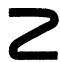
\includegraphics[keepaspectratio]{images/part001_35d0c9a3.jpg}}

Subgroups and quotient groups of a unimodular group are not always unimodular ( \(\S2\) , Exer. 5). See, however, Prop. 10 of \(\S2\) , No.~7.

*We shall see later that semi-simple or nilpotent connected Lie groups are unimodular.*

